\documentclass[10pt]{article}

\usepackage[margin=1in]{geometry}
\usepackage{graphicx}
\usepackage{xspace}
\usepackage{amsmath}
\usepackage[normalem]{ulem}
\usepackage{xcolor}
\usepackage{tikz}

\newcommand{\nt}[1]{\ensuremath{\langle \mathit{#1} \rangle}}
\newcommand{\tm}[1]{\texttt{#1}}

\begin{document}

\title{Quandary Language and Runtime Specification}
\author{Mike Bond}
\maketitle

\newcommand\productions[3]{\nt{#1} ::= \= #2\\#3\smallskip\\}
\newcommand\alt[1]{\> $|$ \' #1 \\}
\newcommand\comment[1]{\` \textcolor{darkgray}{// #1}}

\newcommand\heap[1]{\textcolor{brown}{#1}}
\newcommand\concurrency[1]{\textcolor{blue}{#1}}
\newcommand\mutation[1]{\textcolor{red}{#1}}

\section{Context-free grammar, with notes about semantics}

Colors denote productions used only for
\heap{heap} (including the \tm{Q} and \tm{Ref} types),
\concurrency{concurrency}, and
\mutation{mutation}.
Later, the list of built-in functions uses the same color coding.

\begin{tabbing}
\productions{program}{\nt{funcDefList}}{}

\productions{funcDefList}{\nt{funcDef} \nt{funcDefList}}{
    \alt{$\epsilon$}
}

\productions{funcDef}{\nt{varDecl} \tm{(} \nt{formalDeclList} \tm{)} \tm{\{} \nt{stmtList} \tm{\}}}{}

\productions{varDecl}{\nt{type} \tm{IDENT} \comment{Variables and functions are immutable by default}}{
    \alt{\mutation{\tm{mutable} \nt{type} \tm{IDENT}} \comment{Mutable vars can be updated; mutable funcs can perform updates}}
}

\productions{type}{\tm{int} \comment{64-bit signed integer}}{
    \alt{\heap{\tm{Ref}} \comment{Reference to a heap object with left and right fields of type \tm{Q}; or \tm{nil}}}
    \alt{\heap{\tm{Q}} \comment{Super type of \tm{int} and \tm{Ref}}}
}

\productions{formalDeclList}{\nt{neFormalDeclList}}{
    \alt{$\epsilon$}
}

\productions{neFormalDeclList}{\nt{varDecl} \tm{,} \nt{neFormalDeclList}}{
    \alt{\nt{varDecl}}
}

\productions{stmtList}{\nt{stmt} \nt{stmtList}}{
    \alt{$\epsilon$}
}

\productions{stmt}{\nt{varDecl} \tm{=} \nt{expr} \tm{;} \comment{Declare and initialize variable}}{
    \alt{\mutation{\tm{IDENT} \tm{=} \nt{expr} \tm {;}} \comment{Update to already-declared-and-initialized (mutable) variable}}
    \alt{\tm{if} \tm{(} \nt{cond} \tm{)} \nt{stmt}}
    \alt{\tm{if} \tm{(} \nt{cond} \tm{)} \nt{stmt} \tm{else} \nt{stmt}}
    \alt{\mutation{\tm{while} \tm{(} \nt{cond} \tm{)} \nt{stmt}} \comment{Pointless without mutation}}
    \alt{\mutation{\tm{IDENT} \tm{(} \nt{exprList} \tm{)} \tm{;}} \comment{\tm{IDENT} must be mutable function}}
    \alt{\heap{\tm{free} \nt{expr} \tm{;}} \comment{Frees memory iff explicit memory management enabled}}
    \alt{\tm{return} \nt{expr} \tm{;}}
    \alt{\tm{\{} \nt{stmtList} \tm{\}}}
}

\productions{exprList}{\nt{neExprList}}{
    \alt{$\epsilon$}
}

\productions{neExprList}{\nt{expr} \tm{,} \nt{neExprList}}{
    \alt{\nt{expr}}
}

\productions{expr}{\heap{\tm{nil}} \comment{Special constant value of type \tm{Ref}}}{
    \alt{\tm{INTCONST} \comment{64-bit signed integer of type \tm{int}}}
    \alt{\tm{IDENT}}
    \alt{\tm{-} \nt{expr}}
    \alt{\heap{\tm{(} \nt{type} \tm{)} \nt{expr}} \comment{Explicit downcast from \tm{Q} to \tm{int} or \tm{Ref}}}
    \alt{\tm{IDENT} \tm{(} \nt{exprList} \tm{)}}
    \alt{\nt{binaryExpr}}
    \alt{\concurrency{\tm{[} \nt{binaryExpr} \tm{]}} \comment{Evaluates the left and right sides of the binary expression concurrently}}
    \alt{\tm{(} \nt{expr} \tm{)}}
}

\productions{binaryExpr}{\nt{expr} \tm{+} \nt{expr}}{
    \alt{\nt{expr} \tm{-} \nt{expr}}
    \alt{\nt{expr} \tm{*} \nt{expr}}
    \alt{\heap{\nt{expr} \tm{.} \nt{expr}} \comment{Evaluates to a \tm{Ref} referencing a new heap object}}
}

\productions{cond}{\nt{expr} \tm{<=} \nt{expr}}{
    \alt{\nt{expr} \tm{>=} \nt{expr}}
    \alt{\nt{expr} \tm{==} \nt{expr} \comment{For comparing \tm{int} values only}}
    \alt{\nt{expr} \tm{!=} \nt{expr} \comment{For comparing \tm{int} values only}}
    \alt{\nt{expr} \tm{<}  \nt{expr}}
    \alt{\nt{expr} \tm{>}  \nt{expr}}
    \alt{\nt{cond} \tm{\&\&} \nt{cond}}
    \alt{\nt{cond} \tm{||} \nt{cond}}
    \alt{\tm{!} \nt{cond}}
    \alt{\tm{(} \nt{cond} \tm{)}}
}

\end{tabbing}

\paragraph{Lexical analysis:}

An \tm{IDENT} is a sequence of letters, digits, and underscores such that
the first character is not a digit.

If an \tm{INTCONST} exceeds the bounds of a 64-bit signed integer,
the interpreter's behavior is undefined.

Quandary's syntax is case sensitive.

Quandary allows Java/C/C++-style ``block'' comments \textsf{/* like this */}

\section{Precedence and dangling \tm{else}}

Precedence of operators in high-to-low order:

\begin{enumerate}

\item Expressions in parentheses (\tm{()}) or brackets (\tm{[]})
\item \tm{-} used as a unary operator and \tm{(} \nt{type} \tm{)} (downcast operator)
\item \tm{*}
\item \tm{-} used as a binary operator and \tm{+}
\item \tm{.}
\item \tm{<=}, \tm{>=}, \tm{==}, \tm{!=}, \tm{<}, and \tm{>}
\item \tm{!}
\item \tm{\&\&} and \tm{||}

\end{enumerate}
% %
All operators are left assocative.

Dangling \tm{else} ambiguity is resolved by matching an \tm{else} with the nearest \tm{if} statement allowed by the grammar.

\section{Static typing rules}

The Quandary interpreter checks the following rules prior to executing the program.

\paragraph{Declarations:}

A program must not define a function with the same name as another function, including the built-in functions.
A function must not declare a variable with the same name as a variable that has been defined earlier (including as a parameter)
in the same or an outer/contiaining lexical scope (demarcated by curly braces, i.e., \tm{\{\}},
or by being a single conditional statement in an \textsf{if}/\textsf{else} statement or \textsf{while} loop).
An expression may only access variables declared within the same or an outer/containing 1exical scope.
\emph{Thus for any variable name $v$ at any program point, either $v$ can be accessed or declared, but never both.}

A program must define a function named \tm{main} that takes a single argument of type \tm{int}.

\paragraph{Types and conversions:}

Function calls must have the same number of actuals as the function definition's number of formals.

All \nt{expr} evaluation---including function actuals, return values,
and \tm{free} statements---must be statically type-checked as much as possible,
according to the following type hierarchy:

\begin{center}
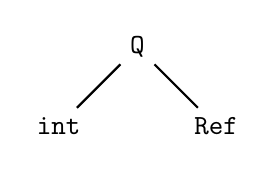
\begin{tikzpicture}
    \node (Q) at (0,0) {\tm{Q}};
    \node (int) at (-1, -1) {\tm{int}};
    \node (Ref) at (1, -1) {\tm{Ref}};

    \draw [thick] (Q) -- (int);
    \draw [thick] (Q) -- (Ref);
\end{tikzpicture}
\end{center}
% %
Both silent and explicit upcasts and flat-casts are permitted.
Downcasts require an explicit cast (\nt{expr} ::= \tm{(} \nt{type} \tm{)} \nt{expr}), which is checked at run time.

\paragraph{Immutability:}

Variables and functions are \emph{immutable} unless declared as \tm{mutable}.
An immutable variable must not be the
assigned-to variable in an assignment statement
(\nt{stmt} ::= \tm{IDENT} \tm{=} \nt{expr} \tm {;}).

An immutable function's body must not contain
calls to \tm{mutable} functions (including built-in \tm{mutable} functions).

A call statement must call a \tm{mutable} function.

\paragraph{Miscellaneous:}

Each function must be statically guaranteed to return a value.
The interpreter's static checking may verify this property
by simply checking that the interpreter's last statement is a
\tm{return} statement (and reporting an error if not).

A function may also contain earlier \tm{return} statements,
including \tm{return} statements that make code statically unreachable.
In general, statically unreachable code is not erroneous.

\section{Built-in functions}

\heap{\tm{Q left(Ref r)} -- Returns the left field of the object referenced by \tm{r}} \\
\\
\heap{\tm{Q right(Ref r)} -- Returns the right field of the object referenced by \tm{r}} \\
\\
\heap{\tm{int isAtom(Q x)} -- Returns \tm{1} if \tm{x} is \tm{nil} or an \tm{int}, and \tm{0} otherwise (it is a \tm{Ref})} \\
\\
\heap{\tm{int isNil(Q x)} -- Returns \tm{1} if \tm{x} is \tm{nil}; returns \tm{0} otherwise (it is an \tm{int} or \tm{Ref})} \\
\\
\mutation{\tm{mutable int setLeft(Ref r, Q value)} -- Sets the left field of the object referenced by \tm{r} to \tm{value}, and returns \tm{1}} \\
\\
\mutation{\tm{mutable int setRight(Ref r, Q value)} -- Sets the right field of the object referenced by \tm{r} to \tm{value}, and returns \tm{1}} \\
\\
\concurrency{\tm{mutable int acq(Ref r)} -- Acquires the lock of the object referenced by \tm{r} and returns \tm{1}} \\
\\
\concurrency{\tm{mutable int rel(Ref r)} -- Releases the lock of the object referenced by \tm{r} and returns \tm{1}} \\
\\
\tm{int randomInt(int n)} -- Returns a random \tm{int} in $[0,n)$ \\

\section{Language semantics and operation of the interpreter}

The interpreter executes the defined function called \tm{main}
and passes a command-line parameter as \tm{main}'s argument:

\begin{verbatim}
  $ ./quandary
  Expected format: quandary [OPTIONS] QUANDARY_PROGRAM_FILE INTEGER_ARGUMENT
  Options:
    -gc (MarkSweep|MarkSweepVerbose|RefCount|Explicit|NoGC)
    -heapsize BYTES
  BYTES must be a multiple of the word size (8)
\end{verbatim}
% %
The interpreter prints the return value of \tm{main} in the following way:

\begin{verbatim}
  Interpreter returned ((5 . nil) . (-87 . (9 . 3)))
\end{verbatim}
% %
Incorrect command-line parameters, including \texttt{QUANDARY\_PROGRAM\_FILE} not being found,
have undefined behavior (i.e., the interpreter may fail in any way).

\paragraph{Function calls:}

Function call semantics are pass-by-value.

\paragraph{Order of evaluation:}

The interpreter evaluates expressions in left-to-right order, i.e.,
it evaluates the left side of (non-concurrent) binary expressions before the right side,
and it evaluates function call actual expressions in left-to-right order.

Binary boolean operators (\tm{\&\&} and \tm{||}) use short-circuit evaluation.

\paragraph{Dynamic type checking:}

The interpreter should check executed type downcasts and report a fatal error
on a type downcast failure.

\paragraph{\tm{nil} dereference:}

Calling \tm{left()}, \tm{right()}, \tm{setLeft()}, or \tm{setRight()}
with a first argument of \tm{nil} should cause a fatal run-time error.

\paragraph{Heap mutation:}

A new heap object's left and right fields are each initialized to
an \tm{int} or \tm{Ref} value,
and must remain as either an \tm{int} or \tm{Ref} value, respectively,
for the duration of the execution.
Thus the interpreter should fail with a dynamic type checking error if
the \tm{setLeft()} or \tm{setRight()} function
attempts to overwrite an \tm{int} slot with a \tm{Ref} value,
or a \tm{Ref} slot with an \tm{int} value.
This restriction avoids the implementation challenge of performing accesses
to a field, which would require updating both the value and associated type metadata atomically.

\paragraph{Memory management:}

An execution should report an ``out of memory'' error if and only if the non-freed memory exceeds the specified maximum heap size.

The interpreter potentially supports explicit memory management
and mark--sweep and reference counting garbage collection
(and optionally others as well, e.g., semi-space). See command-line arguments above.

Explicit memory management only:
An execution that accesses a freed object has undefined semantics.
An execution that performs double-free on a reference has undefined semantics.
An execution that tries to free \tm{nil} has undefined semantics.

Trace-based garbage collection only:
An evaluation of an allocation expression
(\nt{binaryExpr} ::= \nt{expr} \tm{.} \nt{expr})
performs trace-based GC when and only when the non-freed memory exceeds the specified maximum heap size.
Trace-based GC frees objects that are transitively unreachable from the roots (functions' local variables and intermediate values).
Implementing support for stopping multiple threads at GC-safe points is not required;
if trace-based GC is triggered when multiple threads are active,
the interpreter has undefined behavior (but ideally it will report an error, to help with debugging).

\paragraph{Concurrency:}

A concurrently evaluated binary expression
\tm{[} \nt{binaryExpr} \tm{]}
evaluates the left and right child expressions in two new concurrent threads (i.e., thread fork),
and waits for both threads to finish (i.e., thread join).

Thread fork and join and lock acquire and release are synchronization operations that induce happens-before edges.
Conflicting accesses unordered by happens-before constitute a data race.

An execution of a program with a data race has undefined semantics.
An execution in which a thread performs a \tm{rel()} of a lock it does not hold, has undefined semantics.

\paragraph{Error checking:}

To help with grading, the interpreter \emph{process} should return one of the following error codes as appropriate:

\begin{itemize}
\item 0 -- success
\item 1 -- lexical analysis or parsing error
\item 2 -- static checking error
\item 3 -- dynamic type checking error
\item 4 -- \tm{nil} dereference error
\item 5 -- Quandary heap out-of-memory error
\end{itemize}
% %
The interpreter script (\texttt{quandary}) should print this return code.
Specifically, the script should handle executions as follows.

\begin{enumerate}

\item For a non-erroneous, terminated program,
the script should print the following as its last two lines:
% %
\begin{verbatim}
  Interpreter returned RETURN_VALUE_OF_MAIN
  Quandary process returned 0
\end{verbatim}
% %
where \texttt{RETURN\_VALUE\_OF\_MAIN} is return value of the Quandary program's \texttt{main} function.

Printing anything before that is fine.

\item For a non-erroneous, non-terminating execution (e.g., a program execution with an infinite loop),
the script should not terminate. Printing anything is fine.

\item For an execution that should return error code \texttt{ERROR\_CODE},
the script should print the following as its last line:
% %
\begin{verbatim}
  Quandary process returned ERROR_CODE
\end{verbatim}
% %
Printing anything before that is fine.

\item For an execution that has undefined behavior, any behavior and output is fine (including uncaught exceptions).
An interpreter can safely assume that programs and inputs with undefined behavior will \emph{not} be executed.

\end{enumerate}
% %
If the \emph{interpreter program itself} runs out of stack memory,
runs out of heap memory, or allocates too many threads,
then behavior is undefined (any behavior is acceptable).
For a reasonable Quandary input program,
the interpreter should succeed if given enough stack memory,
heap memory, and thread count limit.

\section{Implementing the interpreter}

An interpreter written in Java or C++ should allocate heap objects
into raw memory (represented by a primitive array in Java, for example),
and assume that raw memory provides only low-level load, store, and compare-and-set operations.
When writing the interpreter, use the provided \tm{Heap} class to emulate raw memory.

\end{document}
